% !TEX program = lualatex
% LaTeX template for ECE 486 Lab

\documentclass[a4paper]{article}
\usepackage{indentfirst}
\usepackage{fancyhdr}
\usepackage{enumerate}
\usepackage{fontenc}
\usepackage{graphicx}
\usepackage{caption}
\usepackage{mathtools} % load AMS maths
\usepackage{amsmath}  % for math spacing
\usepackage{amssymb}  % for math spacing
\usepackage{fontspec}
\usepackage{lastpage}
\usepackage[margin=1in]{geometry} % an easy way to change page layout
                                  % Thanks to Brady Salz 
\setlength{\parskip}{1em} % 设置段落间距
% ----------------------------
%            Tikz
% ----------------------------

\usepackage{tikz}
\usetikzlibrary{shapes,arrows}
\usepackage{verbatim}

% ----------------------------

% \usepackage{kpfonts-otf}
% \usepackage{libertinus-otf}
% \usepackage{plex-otf}
\newcommand{\D}{\text{d}}

\usepackage{mathptmx}
\setmainfont{Times New Roman}

\newcommand{\score}{\hfill \underline{\hspace{0.65cm}}\,/} % for score underline
\newcommand\RR{\textsuperscript{\textregistered}~} % for registered mark
\newcommand{\EXERCISE}[1]{\subsection*{Ex \textit{#1}.}}
\newcommand{\EXERCISENAME}[2]{\subsection*{Ex #1: \textit{#2}}}
\newcommand\makeMyTitle{\maketitle \thispagestyle{firstPage}}

\pagestyle{fancy}
\fancyhf{}
\fancyhead[C]{}
\fancyhead[L]{\it Lab \LABNUMBER: \LABTITLE}
\fancyhead[R]{\it \today}
\fancyfoot[L]{\textit{Tiantian Zhong}}
\fancyfoot[C]{\thepage/\pageref{LastPage}}
\fancyfoot[R]{\textit{0000000000}}
\renewcommand{\headrulewidth}{0.5pt}
\renewcommand{\footrulewidth}{0.5pt}

\fancypagestyle{firstPage}{
    \fancyhf{}
    \fancyhead[L]{\it ECE 486 \\\it Control Systems}
    \fancyhead[C]{}
    \fancyhead[R]{\it Fall 2022 \\\it  ZJU-UIUC Institute}
    \fancyfoot[L]{}
    \fancyfoot[C]{\thepage/\pageref{LastPage}}
    \fancyfoot[R]{}
    \renewcommand{\headrulewidth}{0.5pt}
    \renewcommand{\footrulewidth}{0.5pt}
}

\newcommand{\E}{\text{e}}
% \newcommand{\Diff}{\text{d}}
\renewcommand{\Re}{\text{Re}}
\renewcommand{\Im}{\text{Im}}

\title{\textbf{Lab Report} \\ Lab \#\LABNUMBER: \textsc{\LABTITLE}}
\author{\AUTHOR \\ \ID}
\date{\today}

\def\AUTHOR{Tiantian Zhong}
\def\ID{3200110643}
% \def\REPORTTITLE{\textsc{\LABTITLE}}

\everymath{\displaystyle}

% ----------------------------
%      Tikz Configuration
% ----------------------------

\tikzstyle{block} = [draw, rectangle, 
minimum height=3em, minimum width=3em]
\tikzstyle{sum} = [draw, circle, node distance=1cm]
\tikzstyle{input} = [coordinate]
\tikzstyle{output} = [coordinate]
\tikzstyle{pinstyle} = [pin edge={to-,thin,black}]
\tikzstyle{triangle} = [isosceles triangle, draw, minimum height = 3em]
\newcommand\K{\text{k}} % kilo = 1000
\date{    \begin{tabular}{rl}
    Experiment Date: &  \EXPDATE \\
    Report Date: & \RPTDATE
\end{tabular} }

\def\LABNUMBER{3}
\def\LABTITLE{Digital Simulation of a Closed-Loop System}
\def\RPTDATE{\today}
\def\EXPDATE{October 25, 2022}


\begin{document}
    \makeMyTitle
   
    \section*{\sc Prelab Exercises}
    \EXERCISE{a}
    The block diagram is shown as Figure \ref{fig-block}, \ref{fig-torque-motor}, and \ref{fig-tape-dynamics}.

    \begin{figure}[h!]
        \begin{minipage}{0.99\linewidth}
            \centering
            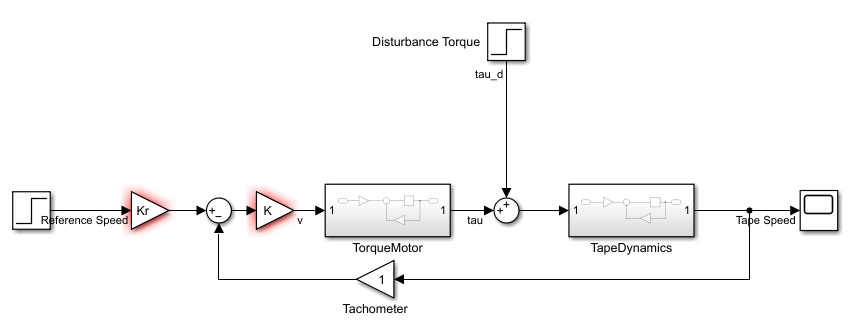
\includegraphics[width=0.99\textwidth]{figs/prelab-block-overall.png}
            \caption{Block Diagram for the System}
            \label{fig-block}
        \end{minipage}
        \\
        \begin{minipage}{0.48\linewidth}
            \centering
            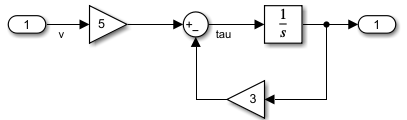
\includegraphics[width=0.99\textwidth]{figs/prelab-block-torque-motor.png}
            \caption{Block Diagram for Torque Motor Subsystem}
            \label{fig-torque-motor}
        \end{minipage}
        \hspace{2em}
        \begin{minipage}{0.48\linewidth}
            \centering
            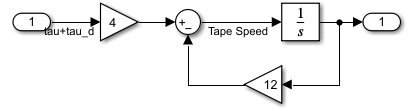
\includegraphics[width=0.99\textwidth]{figs/prelab-block-tape-dynamics.png}
            \caption{Block Diagram for Tape Dynamics Subsystem}
            \label{fig-tape-dynamics}
        \end{minipage}
    \end{figure}

    \EXERCISE{b}

    The system can be represented with, in $s$-domain,
    \begin{equation}
        \Omega = \left[(\Omega_r K_r - \Omega)KH_1+T_d\right]H_2
    \end{equation}
    where $H_1$ and $H_2$ are the transfer function for Torque Motor and Tape Dynamics, respectively.

    Using the conditions given, we derive the transfer functions $H_1$ and $H_2$ as
    \begin{align}
        H_1(s) &= \frac{T(s)}{V(s)} = 5\cdot \frac{3}{s(s+3)} \cdot \frac{1}{\frac{1}{s}}=\frac{15}{s+3} \\
        H_2(s) &= \frac{\Omega(s)}{T(s)+T_d(s)} = \frac{1}{\frac{1}{4}s+3} = \frac{4}{s+12}
    \end{align}

    As we take $\tau_d=0$, whose Laplace transform should be $T_d = \mathcal{L} \left\lbrace \tau_d \right\rbrace = 0$, we will find
    \begin{equation}
        \frac{\Omega(s)}{\Omega_r(s)} = \frac{K_r\Omega_r K H_1 H_2}{K H_1 H_2 +1} = \boxed{\frac{60K\cdot K_r}{s^2+15s+60K+36}} (\tau_d = 0)
        \label{eq-omega-r}
    \end{equation}

    With $\omega_r=0 \leftrightarrow \Omega_r = 0$, we derive the ratio of tape speed and disturbance torque as 
    \begin{equation}
        \frac{\Omega(s)}{T_d(s)}=\frac{H_2}{KH_1 H_2 +1} = \boxed{\frac{4s+12}{s^2 +15s+60K+36}} (\omega_r = 0)\label{eq-omega}
    \end{equation}

    \EXERCISE{c}

    Solve for poles of the system and we have
    \begin{equation}
        s_{\text{pole}}=\frac{-15\pm \sqrt{15^2-4(60K+36)}}{2}=\frac{-15\pm \sqrt{81-240K}}{2},
    \end{equation}
    all of which have to be located on OLHP. This indicates that 
    \begin{align}
            81-240K &< 0 \\
            \Re(s_{\text{poles}}) &< 0 \\
            60K+36&>0 \notag \\
            K\cdot K_r &>0 \notag
    \end{align}
    
    Thus $\boxed{K>\frac{81}{240}=\frac{27}{80}}$.

    \EXERCISE{d}
    With Equation \ref{eq-omega}, we pull in $T_d = \frac{1}{s}$ and $\omega\leq 0.01\leftrightarrow \Omega \leq \frac{0.01}{s}$ and the FVT gives
    \begin{align}
        \Omega_{\text{ss}}(s)=\lim_{s\rightarrow 0} \Omega (s) &= \lim_{s\rightarrow 0} \frac{60K\cdot K_r}{s^2 + 15s + 60K+ 36}\cdot \frac{1}{s} \notag\\
        &= \frac{60K\cdot K_r}{60K+36}\cdot \frac{1}{s}\leq \frac{0.01}{s}
    \end{align}
    which yields $\boxed{K \leq \frac{0.03}{5K_r -0.05}}$.

    \EXERCISE{e}
    The solution for $\Omega_r = \frac{1}{s}$ gives
    % \begin
\end{document}